
\subsection{Media}
\paragraph{}
After \textit{geometry} the most natural section to discuss in the input card is the \textit{Media} section. In this section, materials are defined if they aren't in the FLUKA default material database and they're assigned to regions. There are four main types of cards in this section: \textcolor{Maroon}{MATERIAL}, \textcolor{Maroon}{COMPOUND}, \textcolor{Maroon}{ASSIGNMA}, and \textcolor{Maroon}{LOW-MAT}. 

\begin{figure}[h]
    \begin{center}
    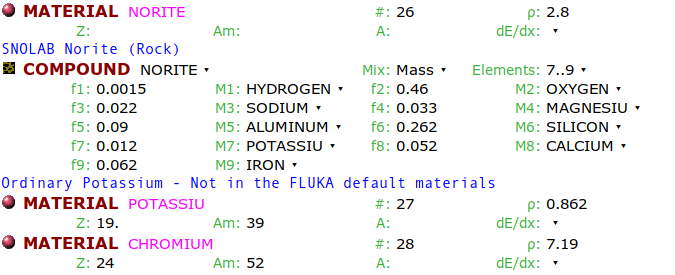
\includegraphics[scale=0.5]{figures/media_1.png}
    \caption{A subset of the media section in the input file}
    \label{fig:media1}
    \end{center}
\end{figure}

\paragraph{}
First, referring to figure \ref{fig:media1} and describe the first card in the media section. It is a \textcolor{Maroon}{MATERIAL} card with variable name \textcolor{magenta}{NORITE}. This card declares a new material called \textcolor{magenta}{NORITE} which is given a density, and a user-chosen material number for later reference \footnote{The numbers for user-defined materials can't start at 1, they proceed from the last number of the native FLUKA materials list (25)}. Norite rock is an abundant rock around the Sudbury basin. It is a mixture of various elements and must therefore be defined with the subsequent \textcolor{magenta}{COMPOUND} card. The arguments for this card are the component materials of the compound and their respective fractions by mass, volume, or atom abundance. These arguments should be very clear, the odd one out is \textcolor{ForestGreen}{Elements} which simply allows for the resizing of the compound card to accomodate more or fewer elements. The following cards, \textcolor{magenta}{POTASSIU} and \textcolor{magenta}{CHROMIUM} are necessary to define as they are not in the default FLUKA materials list. Given that these are elemental, we must provide the arguments of atomic number (\textcolor{ForestGreen}{Z}), the atomic mass (\textcolor{ForestGreen}{Am}) in g/mol, and the atomic mass number (\textcolor{ForestGreen}{A}) which is assumed to be the most abundant for the given (\textcolor{ForestGreen}{Z}) if left unspecified. Of course \textcolor{ForestGreen}{$\rho$} is the density, and \textcolor{ForestGreen}{$dE/dx$} allows to select another material to use for the case of ionization— we do not use this feature.

\paragraph{}
Once all the materials are defined they are then assigned to regions with the \textcolor{Maroon}{ASSIGNMA} cards. This card a list of arguments including the material to be assigned and the regions it will be assigned to. One of these cards can assign a material to several regions, however, the regions had to have been declared in some regular order for this to work for multiple regions. That is, a user might wish to have every region from the first to last of N regions to be full of water. In this case, the card would have arguments \textcolor{ForestGreen}{Reg:} $=$ 1 and \textcolor{ForestGreen}{to Reg:} $= N$. Alternatively, a user can assign a material to every $k^{\text{th}}$ region in the range $[1,N]$ by setting \textcolor{ForestGreen}{Step:} $=$ 3. This seems like a strange and uncomfortable way to do things because any modification to the region declarations can totally offset the material assignments. Nevertheless, it is how it works. In the ``nEXO\_OD.inp'' input file, each region is assigned a material separately and by name. This issue ought not occur.

\subsubsection{Specific Materials}
\paragraph{}
Now that the media input options have been discussed, we will overview some of the materials used in the ``nEXO\_OD.inp'' input file as these may not be an exact representation of the material structure of nEXO. First, the rock surrounding the geometry is of a particular variety that is very common around SNOLAB: norite. Its composition is shown in the table below. Then, another compound used in the configuration is HFE, the refrigerant in the inner cryostat whose composition is shown in the table below. 

\begin{center}
    \label{tab:norite}
    \begin{tabular}[h]{|c|c|}
        \hline
        \multicolumn{2}{|c|}{Norite $\rho = 2.894 $ g/cm$^3$} \\
        \hline
        \hline
        Element & Atomic Composition (\%) \\
        \hline
        O & 46.0 \\
        Si & 26.2 \\
        Al & 9.0 \\
        Fe & 6.2 \\
        Ca & 5.2 \\
        Mg & 3.3 \\
        Na & 2.2 \\
        K & 1.2 \\
        Ti & 0.5 \\
        H & 0.15 \\
        Mn & 0.1 \\
        C & 0.04 \\
        \hline
    \end{tabular}
    \quad
    \label{tab:HFE}
    \begin{tabular}[h]{|c|c|}
        \hline
        \multicolumn{2}{|c|}{HFE $\rho \approx 1.5 $ g/ml} \\
        \hline
        \hline
        Element & Atomic Composition (\%) \\
        \hline
        F & 46.6 \\
        C & 26.7 \\
        H & 20.0 \\
        O & 6.7 \\
        \hline
    \end{tabular}
\end{center}
